\documentclass[xcolor=table, aspectratio=169]{beamer}
%\documentclass{beamer}
\title[Machine Learning and AI]{Fin 395 4 Lecture 3: \\ Machine Learning and Artificial Intelligence}
\author[Empirical Asset Pricing (Johnson)]{Professor Travis Johnson \\ The University of Texas at Austin}
\date{}

\mode<presentation> {
\usetheme{Singapore}
%\usecolortheme{beaver}
% or g...
\setbeamercovered{transparent}
% or whatever (possibly just delete it)
\setbeamertemplate{navigation symbols}{}
\setbeamertemplate{headline}{}
\usefonttheme{professionalfonts}

\definecolor{schoolcolor1}{RGB}{191,87,0}
\definecolor{schoolcolor2}{RGB}{255,255,255}
\definecolor{alertschoolcolor}{RGB}{191,87,0}

\setbeamercolor{alerted text}{fg=alertschoolcolor}
\setbeamercolor*{palette primary}{fg=schoolcolor2,bg=schoolcolor1}
\setbeamercolor*{palette secondary}{fg=white,bg=schoolcolor2}

\setbeamercolor*{sidebar}{fg=white,bg=black}

\setbeamercolor*{palette sidebar primary}{fg=schoolcolor1!10!black}
\setbeamercolor*{palette sidebar secondary}{fg=white}
\setbeamercolor*{palette sidebar tertiary}{fg=schoolcolor1!50!black}
\setbeamercolor*{palette sidebar quaternary}{fg=gray}

\setbeamercolor*{titlelike}{parent=palette primary}
\setbeamercolor{frametitle}{fg=schoolcolor2,bg=schoolcolor1}

\setbeamercolor*{separation line}{}
\setbeamercolor*{fine separation line}{}

\setbeamercolor{itemize item}{fg=schoolcolor1,bg=white}
\setbeamercolor{itemize subitem}{fg=schoolcolor1,bg=white}
\setbeamercolor{enumerate item}{fg=schoolcolor1,bg=white}

\newcommand{\alertbf}[1]{\alert{\textbf{#1}}}

%\setbeamertemplate{footline} % To remove the footer line in all slides uncomment this line
% \setbeamertemplate{footline}[page number] % To replace the footer line in all slides with a simple slide count uncomment this line
\setbeamertemplate{itemize subitem}[triangle]
}

\usepackage{multicol}
\usepackage{bigstrut}
\usepackage{multirow}
\usepackage{verbatim}
\usepackage{amsmath, amsthm, amssymb}
\usepackage{etex}
\usepackage[all]{xy}
\usepackage{eurosym}
\usepackage{array}
\usepackage{tikz}
\usepackage{chronology}
\usepackage{changepage}
\usepackage{booktabs}
\usepackage{framed}
\usepackage{onimage}
\usepackage{changepage}
\usepackage{listofitems} % for \readlist to create arrays
\tikzstyle{mynode}=[thick,draw=blue,fill=blue!20,circle,minimum size=22]
%\usepackage{pdfpages}
%\usepackage{xy}

\newcommand{\Q}{\mathbb{Q}}
\newcommand{\oo}{\emptyset}
\newcommand{\Y}{\mathcal{Y}}
\newcommand{\X}{\mathcal{X}}
\newcommand{\bX}{\mathbf{X}}
\newcommand{\E}{\mathbb{E}}
\newcommand{\I}{\mathbf{I}}
\newcommand{\T}{\mathcal{T}}
\newcommand{\f}{\mathnormal{f}}
\newcommand{\R}{\mathbb{R}}
\newcommand{\Z}{\mathbb{Z}}
\newcommand{\C}{\mathbb{C}}
\newcommand{\N}{\mathbb{N}}
\newcommand{\B}{\mathcal{B}}
\newcommand{\s}{\bar{s}}
\newcommand{\textepsilon}{\epsilon}

\DeclareMathOperator*{\argmin}{arg\,min}


%\pgfpagesuselayout{1 on 1 with notes}[letterpaper,border shrink=25mm]

\definecolor{lightgray}{gray}{0.9}

\newenvironment{changemargin}[2]{%
  \begin{list}{}{%
    \setlength{\topsep}{0pt}%
    \setlength{\leftmargin}{#1}%
    \setlength{\rightmargin}{#2}%
    \setlength{\listparindent}{\parindent}%
    \setlength{\itemindent}{\parindent}%
    \setlength{\parsep}{\parskip}%
  }%
  \item[]}{\end{list}}

\usetikzlibrary{arrows,positioning} 
\tikzset{
    %Define standard arrow tip
    >=stealth',
    %Define style for boxes
    punkt/.style={
           rectangle,
           rounded corners,
           draw=black, very thick,
           %text width=8.5em,
           minimum height=2em,
           text centered},
    % Define arrow style
    pil/.style={
           ->,
           thick,
           shorten <=2pt,
           shorten >=2pt,}
}

\newcommand*\oldmacro{}%
\let\oldmacro\insertshorttitle%
\renewcommand*\insertshorttitle{%
  \oldmacro\hfill%
  \insertframenumber}

\def\arraystretch{0.9}
\setlength{\tabcolsep}{2.5pt}
\setbeamercovered{transparent}

\begin{document}
\begin{frame}
  \titlepage 
\end{frame}


% Objectives slide (user provided)
\begin{frame}{Objectives for today}
    \begin{enumerate}
        \item What is \alertbf{machine learning}, and how do the core methodologies work?
        \item How can we use machine learning in finance \& asset pricing?
        \item What are some example applications? 
    \end{enumerate}

    \vspace{0.5cm}

    \begin{enumerate}
    \setcounter{enumi}{3}
        \item What is \alertbf{AI} and how does it relate to machine learning?
        \item How can we leverage AI to be better researchers?
    \end{enumerate}
\end{frame}

\begin{frame}{Machine learning definition}
    What is \alertbf{machine learning}? Gu, Kelly, and Xiu (2020) define it as:

    \begin{enumerate}
        \item {\small``a diverse collection of high-dimensional models for statistical prediction, combined with}
        \item {\small so-called `regularization' methods for model selection and mitigation of overfit, and}
        \item {\small efficient algorithms for searching among a vast number of potential model specifications.''}
    \end{enumerate}


    ~

    Key difference from standard econometrics: \alertbf{prediction} ($\hat{y}$) instead of \alertbf{parametric hypothesis testing} ($\hat{\beta}=0$)

    ~

    Machine learning well-suited to some \alertbf{asset pricing} problems:
    \begin{enumerate}
        \item Lots of data
        \item Lots of candidate predictors
        \item Measuring moments of data important, less focus on causal effects
    \end{enumerate}
\end{frame}

\begin{frame}{Comparison of econometrics and machine learning: terminology}
    \begin{center}
\begin{tabular}{ll}
\textbf{Econometrics} & \textbf{Machine Learning} \\
\midrule
Estimation & Training, learning, fitting \\
Parameters ($\beta$) & Weights, parameters \\
Regressors, covariates, independent variables & Features \\
Regressand, dependent variable & Target, label \\
Model specification search & Hyperparameter tuning \\
Goodness-of-fit (in-sample) & Performance (out-of-sample) \\
Computing fitted value & Inference \\
Statistical inference (e.g., hypothesis tests, CIs) \hspace{6pt}  & --- \\
Causal inference (e.g., instruments, DiD) & --- \\
Shrinkage, variable selection & Regularization \\
Fixed effect & One-hot feature \\
Objective function & Loss function \\
\midrule
\end{tabular}
    \end{center}
\end{frame}

\begin{frame}{Comparison of econometrics and machine learning: philosophy}
    \begin{center}
\begin{tabular}{lll}
\textbf{Concept} & \textbf{Econometrics} \hspace{2.5cm} & \textbf{Machine Learning} \hspace{2cm} \\
\midrule
Objective & Hypothesis testing & Prediction \\[12pt]
Feature count & & \\[12pt]
Parameter count & & \\[12pt]
Data mining & & \\[12pt]
Key metrics & & \\[12pt]
Assumptions & & \\[12pt]
\midrule

\end{tabular}
    \end{center}
\end{frame}

% Core ML Methodologies: An Overview
\begin{frame}{Overview of core ML methodologies}
The ML literature offers a diverse toolkit for empirical researchers
        \begin{enumerate}
            \item \alertbf{Supervised Learning} (for regression and classification problems)
            \begin{itemize}
                \item We have $X$ and $Y$
            \end{itemize}
            \item \alertbf{Unsupervised Learning} (for clustering and density estimation)
            \begin{itemize}
                \item We only have $X$
            \end{itemize}
            \item \alertbf{Dimension Reduction Techniques} (often used as pre-processing)
            \begin{itemize}
                \item We (usually) only have $X$
            \end{itemize}
        \end{enumerate}

        ~

Focus today primarily on \alertbf{supervised learning} methods: ridge regression, LASSO, elastic net, regression trees/forests, boostings, neural networks

\end{frame}

% Supervised Learning: Regression Problems
\begin{frame}{Supervised learning problem statement}
\alertbf{Goal}: Estimate the conditional mean of $y_i$ given a vector of covariates $X_i$:
\begin{align*}
    \E( y_i | X_i) = f(X_i,\theta),
\end{align*}
where the specification of $f$ and the parameters $\theta$ vary across approaches
    \begin{itemize}
        \item This is a canonical problem in both ML and econometrics
        \item Key differences from traditional econometrics
        \begin{itemize}
            \item $\theta$ can be huge, often larger than the sample size
            \item No presumption that the conditional distribution follows a particular parametric model (e.g. $N(X_i\beta,\sigma_i^2)$)
            \item Derivatives of conditional expectation w.r.t. any covariate is not of intrinsic interest
            \item Focus is on out-of-sample predictions and their accuracy
            \item Allow for possibility that conditional expectation may be an extremely non-monotone function with high-order interactions
        \end{itemize}
    \end{itemize}
\end{frame}

% Supervised Learning: Penalized Linear Models
\begin{frame}[t]{Penalized linear models}
\vspace{-12pt}
\begin{align*}
    \hat{\E}( y_i | X_i) &= X_i \hat{\beta}, &
\hat{\beta} &= \argmin_\beta \sum_{i=1}^N \left( y_i - X_i \beta \right)^2 + \lambda_1 \sum_{k=1}^K \vert \beta_k \vert + \lambda_2 \sum_{k=1}^K \beta_k^2
\end{align*}

Linear model with penalties applies when $\beta$ deviates from zero, designed to ``shrink'' estimates towards an informal prior
    \begin{itemize}
        \item Addresses overfitting, improving OOS performance
        \item When $\lambda_1 > 0$, often wind up at $\beta_k = 0$ corner solution $\Leftrightarrow$ \alertbf{variable selection}
        \begin{itemize}
            \item Helps particularly with `sparsity' -- a bunch of useless variables in $X_i$
        \end{itemize}
        \item When $\lambda_2 > 0$, \alertbf{shrinkage} increasing in deviation from 0
        \begin{itemize}
            \item Helps particularly with `colinearity' -- some elements of $X_i$ are close to a linear combination of other elements
        \end{itemize}
        \item \alertbf{Lasso} (Least Absolute Shrinkage and Selection Operator): $\lambda_1 > 0$, $\lambda_2=0$
        \item \alertbf{Ridge Regression}: $\lambda_1 = 0$, $\lambda_2>0$
        \item \alertbf{Elastic Net}: $\lambda_1 > 0$, $\lambda_2 > 0$
    \end{itemize}
\end{frame}

\begin{frame}{Hyperparameters and cross-validation}
$\lambda_1$ and $\lambda_2$ are our first \alertbf{hyperparameters} -- parameters we must specify rather than directly estimate
\begin{itemize}
    \item Typically passed as parameters in the packages that implement ML algorithms
    \item Practice of trying different hyperparameters is called \alertbf{tuning}
    \item Equivalents in econometrics: number of lags in Newey-West, cluster identifiers, choice of fixed effects, etc.
\end{itemize}

~

\alertbf{Cross-validation} approach splits sample into three:
\begin{enumerate}
    \item \alertbf{Training}: estimate $\theta$ given a set of hyperparameters $\lambda$
    \item \alertbf{Validation}: iterate over possible $\lambda$ values, maximizing performance in this period using forecasts from $\theta$ estimated in training period
    \item \alertbf{Test}: measure performance here using the $\lambda$, $\theta$ estimated using prior periods
\end{enumerate}
For time-series/panel data in asset pricing, we often re-estimate $\theta$, $\lambda$ each year and use the subsequent year as the test sample
    
\end{frame}

% Supervised Learning: Tree-Based Methods I
\begin{frame}[t]{Regression trees}
\vspace{-12pt}
\begin{align*}
    \hat{\E}( y_i | X_i) &= \sum_{k=1}^K\theta_k \mathbf{1}_{X_i \in C_k(L)} & C_k(L) = \prod_{l=1}^L \mathbf{1}_{X_{i,j(l)} \gtrless \overline{X}_{j(l)}}
\end{align*}
Forecast using the sample mean in a segment of the covariate space partition using a sequence of at most $L$ cutoffs applied to one dimension at a time\only<1>{, for example}:  

\only<1>{
~
    \begin{tabular}{cc}
    \includegraphics[width=0.5\linewidth]{Images/gkx_tree1.png} & \includegraphics[width=0.35\linewidth]{Images/gkx_tree2.png}
        \end{tabular}
}
\only<2>{
    \begin{itemize}
        \item Increasing $L$ always increases in-sample fit, may lead to overfitting $\Rightarrow$ we usually penalize this or treat as a hyperparameter
        \item Can capture non-linear relations and interaction effects
        \item When applied to stocks, similar to multi-dimensional \alertbf{portfolio sorts}, but instead of e.g. $3 \times 3 \times 3$ grids we use rectangles are of unequal size
        \item Similar flavor to \alertbf{kernel regression} where you forecast using average of observations ``close enough'' to $X_i$
        \begin{itemize}
            \item Regression lets data tell you what's close enough vs. imposing exogenously
        \end{itemize}
    \end{itemize}
}
\end{frame}

        
        
        
        
        
%         Data are repeatedly split into subsamples based on feature values to predict an outcome [35].
%         \item They capture **individual predictors' nonlinear impact** on expected returns [36].
%         \item \textbf{Random Forests}: An **ensemble method** that combines multiple decision trees [27, 35, 37].
%         \begin{itemize}
%             \item Each tree is built using a **random subsample** of the data and a random subset of features for splitting at each node [35].
%             \item Predictions are then averaged across all trees (e.g., by optimizing out-of-sample performance) [35, 38].
%             \item Reduces variance and overfitting compared to single decision trees [35, 37].
%             \item Can handle **complex nonlinear associations** and a large number of predictor variables [39].
%         \end{itemize}
%         \item Often use measures like **mean-decreased impurity (MDI)** and **mean-decreased accuracy (MDA)** to evaluate feature importance [40, 41].
%     \end{itemize}
% \end{frame}

\begin{frame}[t]{Random forests}
\vspace{-12pt}
\begin{align*}
\hat{\E}( y_i | X_i) &= \frac{1}{M} \sum_{m=1}^M \hat{\E}( y_i | Z_i(m)) & \hat{\E}( y_i | Z_i(m)) &= \sum_{k=1}^K\theta_k \mathbf{1}_{Z_i(m) \in C_{m,k}(L)},
\end{align*}
where $Z_i(m)$ is one of $M$ random smaller-dimensional subsets of $X_i$
\begin{itemize}
    \item \alertbf{Idea:} random trees sometimes overfit by finding tiny subsets with extreme values. Don't let them rely on any one element of $X_i$ too much
    \item One of many \alertbf{ensemble} methods that takes advantage of averaging forecasts across possible models
    \begin{itemize}
        \item `Wisdom of the model crowds'
    \end{itemize}
    \item Results in conditional means that are smoother than a single tree
    \item Generally performs much better than a simple regression tree, one of the best plug-and-play methods because there are relatively few hyperparameters
    \item Can further improve, especially in economics settings, by allowing for local linearity instead of assuming conditional mean is locally constant
\end{itemize}
\end{frame}

\begin{frame}[t]{Boosting and gradient-boosted regression trees}
\vspace{-12pt}
\begin{align*}
    \hat{\E}(y_i | X_i) = \sum_{m=1}^M f_m(X_i,\theta_m) 
\end{align*}
    \alertbf{Boosting} idea: instead of a single complex model $\E( y_i | X_i) = f(X_i,\theta)$ with parameters we estimate all at once, use a sequence of $M$ simple models:
    \begin{align*}
        \E( y_i | X_i) &= f_1(X_i,\theta) \\
        \E( y_i - f_1(X_i,\theta) | X_i) &= f_2(X_i,\theta) \\
        &\cdots \\
        \E( y_i - f_{M-1}(X_i,\theta) | X_i) &= f_M(X_i,\theta),
    \end{align*}
    and form a final composite forecast
    \begin{itemize}
        \item Often used with simple trees with small $L$, called gradient-boosted trees
    \end{itemize}
\end{frame}

% Supervised Learning: Neural Networks I
\begin{frame}[t]{Neural networks: layers, hidden nodes, and activation functions}
\vspace{-12pt}
\begin{align*}
    \hat{\E}(y_i | X_i) = (f_1 \circ f_2 \circ \cdots \circ f_L)(X_i,\theta) 
\end{align*}
\alertbf{Neural networks} are composite functions that map inputs ($X_i$ here) into outputs ($Y_i$ here) using a sequence of operations (\alertbf{layers}) loosely inspired by brain biology\footnote{I focus here on feed-forward neural networks, many other forms exist}

\only<1>{
\makebox[\linewidth][c]{%
    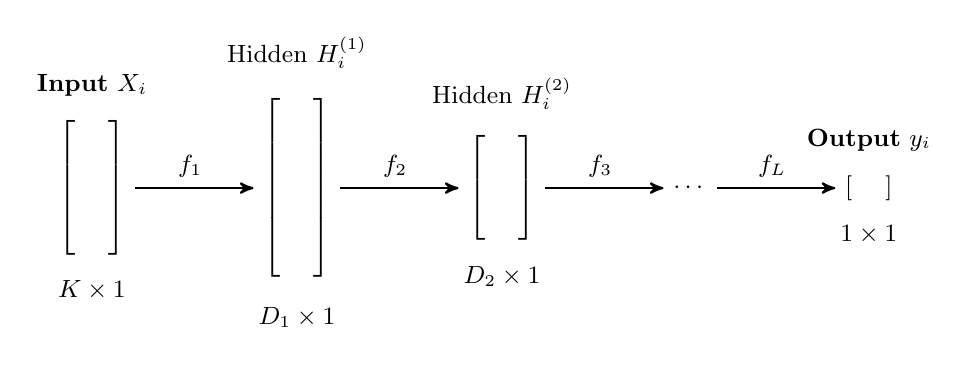
\begin{tikzpicture}[node distance=2cm, font=\small]
    % Input Xi
    \node (xi) {
        $\begin{bmatrix}
             \rule{12pt}{0pt} \\
            \\
            \\
            \\
            \\
        \end{bmatrix}$
    };
    \node[above=0.05cm of xi, align=center] {\textbf{Input} $X_i$};
    \node[below=0.05cm of xi, align=center] {$K \times 1$};
    
    % Hidden 1
    \node[right=1.5cm of xi](h1) {
        $\begin{bmatrix}
            \rule{12pt}{0pt} \\
            \\
            \\
            \\
            \\
            \\
            \\
        \end{bmatrix}$
    };
    \node[above=0.05cm of h1, align=center] {Hidden $H_i^{(1)}$};
    \node[below=0.05cm of h1, align=center] {$D_1 \times 1$};

    % Hidden 2
    \node[right=1.5cm of h1](h2) {
        $\begin{bmatrix}
            \rule{12pt}{0pt} \\
            \\
            \\
            \\
        \end{bmatrix}$
    };
    \node[above=0.05cm of h2, align=center] {Hidden $H_i^{(2)}$};
    \node[below=0.05cm of h2, align=center] {$D_2 \times 1$};

    % dots
    \node[right=1.5cm of h2](dots) {
        $\cdots$
    };

    % Output
    \node[right=1.5cm of dots](yi) {
        $\begin{bmatrix}
            \rule{12pt}{0pt}
        \end{bmatrix}$
    };
    \node[above=0.05cm of yi, align=center] {\textbf{Output} $y_i$};
    \node[below=0.05cm of yi, align=center] {$1 \times 1$};

    \draw[->, thick] (xi.east) -- node[above, align=center]{$f_1$}  (h1.west) ;
    \draw[->, thick] (h1.east) -- node[above, align=center]{$f_2$}  (h2.west) ;
    \draw[->, thick] (h2.east) -- node[above, align=center]{$f_3$}  (dots.west) ;
    \draw[->, thick] (dots.east) -- node[above, align=center]{$f_L$}  (yi.west) ;

    \end{tikzpicture}
}
}
\only<2>
{

~

The functions $f_l$ calculate each element (\alertbf{node}) of a new layer as a linear combination of the nodes in the previous layer with a simple \alertbf{activation function} applied:
\begin{align*}
    H_{i}^{(l)}(j) &= g\left( \theta_0^{l}(j) + \theta^{(l)}(j)' H_i^{(l-1)} \right), \\
    g(z) &= z \mathbf{1}_{z>0} \text{ (or similar function)}
\end{align*}
where $\theta_0^{l}(j)$ is a ``bias'' or intercept term, and $\theta^{(l)}(j)$ is a $D_{l-1} \times 1$ vector of parameters (neurons?)
}
    
\end{frame}

\begin{frame}{Neural networks: layers, hidden nodes, and activation functions}
    \begin{figure}
        \centering
        \includegraphics[width=0.75\linewidth]{Images/nn_illustration.png}
    \end{figure}
\end{frame}

% \begin{itemize}
%         \item \textbf{Neural Networks (NNs)} represent a widespread class of supervised learning methods [46].
%         \item \textbf{Multi-Layer Perceptrons (MLP)}: Consist of at least three layers of nodes: an **input layer**, one or more **hidden layers**, and an **output layer** [47].
%         \item \textbf{Universal Approximators}: MLPs are powerful learning methods that can approximate **virtually any continuous function** with compact support [47-49].
%         \item \textbf{Functional Form Flexibility}: NNs are explicitly designed to approximate **complex nonlinear associations** and interactions, which are critical for situations with ambiguous functional forms [15, 50].
%         \item \textbf{Parameterization}: NNs are parameterized by a vector representation of the vocabulary [51], or weights and biases that are learned from data [52].
%         \item \textbf{Estimation}: Often trained using **stochastic gradient descent** and regularization techniques like Lasso penalty and batch normalization [45, 53, 54].
%     \end{itemize}

\begin{frame}{Properties of neural networks}
    \begin{itemize}
        \item \alertbf{Multi-Layer Perceptrons (MLP)}: any subset of a network consisting of least three layers of nodes: an input layer, one or more hidden layers, and an output layer
        \begin{itemize}
            \item Common setup is to have input -> higher-dimensional hidden -> output as one ``MLP'' stage inside a larger network
        \end{itemize}
        \item \alertbf{Universal approximation}: MLPs are powerful learning methods that, with enough nodes, can approximate virtually any continuous function with only a single hidden layer
        \item \alertbf{Functional form flexibility}: NNs are explicitly designed to approximate complex nonlinear associations and interactions
        \item \alertbf{Parameterization}: loads of parameters, one step in the composite function has $(D_{l-1}+1) D_l$ parameters
        \begin{itemize}
            \item Over a million parameters common even for ``simple'' applications
        \end{itemize}
        \item \alertbf{GPU-friendly}: despite complexity and huge parameter space, mostly just matrix multiplication ($\theta^{(l)} \cdot H_i^{(l-1)}$), gradient easy to calculate
        \begin{itemize}
            \item Modern GPUs optimized to do this very quickly
        \end{itemize}
    \end{itemize}
\end{frame}

% Supervised Learning: Neural Networks II
\begin{frame}{Shallow vs. Deep Learning}
    \begin{itemize}
        \item \alertbf{Shallow Networks}: fewer hidden layers (e.g., one hidden layer)
        \item \alertbf{Deep Networks}: more hidden layers (e.g., three hidden layers or more)
        \item Despite NNs being universal approximators with only one hidden layer, in practice deeper networks typically perform better for the same parameter count
        \item In some asset pricing problems, ``shallow'' learning can outperform ``deeper'' learning, unlike in fields like computer vision
        \begin{itemize}
            \item This is likely due to the comparative dearth of data and low signal-to-noise ratio in asset pricing problems
            \item Neural network performance for individual stock returns often peaks at a moderate number of layers (e.g., three hidden layers) and then declines 
        \end{itemize}
    \end{itemize}
\end{frame}

\begin{frame}{Embedding and Autoencoding}
\alertbf{Embedding} is a map from a high-dimensional, complex input to a lower-dimensional vector output that retains as much information as possible
\begin{itemize}
    \item For simple numeric inputs, this is a form of dimension reduction
    \item For categorical, text, or image inputs this is a more-complex mapping
    \begin{itemize}
        \item Classic example is word embeddings, e.g. ``Word2Vec'', which represents each word as a vector with e.g. 300 dimensions. Gives you cool things like:
        $$\overrightarrow{\text{Sushi}} - \overrightarrow{\text{Japan}} + \overrightarrow{\text{Germany}} \approx \overrightarrow{\text{Bratwurst}} $$
    \end{itemize}
\end{itemize}

~

An \alertbf{autoencoder} learns a lower-dimensional representation of the input vector (form of dimension reduction)
\begin{itemize}
    \item Trained along side a ``decoder'' that restores the original dimensionality, try to match as close as we can
\end{itemize}
\end{frame}

% Unsupervised Learning: Clustering and Density Estimation
{
\setbeamercolor{background canvas}{bg=schoolcolor1}
\begin{frame}
\begin{center}
\large{
\textcolor{white}{BREAK}    
}
\end{center}
\end{frame}
}

% ML in Empirical Asset Pricing: Broad Applications
\begin{frame}{ML in empirical asset pricing: possible applications}
    
\end{frame}

% Stock Return Predictability: Neural Networks (GKX)
\begin{frame}{Stock return predictability}
Canonical measurement problem in asset pricing: estimate
    \begin{align*}
        \E( r_{i,t+1} \vert I_t ),
    \end{align*}
    where $r_{i,t+1}$ is the excess return of asset $i$ and $I_t$ is the unobservable information set of investors at time $t$
    \begin{itemize}
        \item Once measured, can work on understanding its economic determinants
    \end{itemize}

    \vspace{6pt}
    
\alertbf{Gu, Kelly, and Xiu (2019)} show:
\begin{enumerate}
    \item Allowing for non-linearities and interaction effects matters
    \item Value added for machine learning is larger for predicting market/portfolio returns in the time-series than it is for predicting cross-section
    \item Economic gains from machine learning forecasts are large
    \begin{itemize}
        \item 0.77 out-of-sample Sharpe Ratio for market timing strategy, 1.35 for value-weighted long-short strategy
    \end{itemize}
    \item Best predictors are price trends, liquidity, and volatility variables
    \item Strategies have high turnover, overweight microcaps $\Rightarrow$ sensitive to txn costs
\end{enumerate}
\end{frame}

% Bond Return Predictability: NNs with Yields & Macro
\begin{frame}[t]{Bond return predictability}
\alertbf{Bianchi, Büchner, and Tamoni (2021)}: can apply similar methods to measure conditional bond risk premia
    \begin{itemize}
        \item Topic of Jay's presentation today
    \end{itemize}
\end{frame}

% % Stock Return Predictability: Adversarial ML & SDF (CPZ)
% \begin{frame}{Stock Return Predictability: Chen, Pelger, Zhu (}
%     \begin{itemize}
%         \item \textbf{Method}: Chen, Pelger, and Zhu (CPZ) combine **four neural networks**, including two Feed-Forward Networks (FFNs) and two Recurrent Neural Networks (RNNs) with Long Short-Term Memory (LSTM) cells [54, 63].
%         \item \textbf{Objective}: Incorporates a **no-arbitrage condition** by using a **minimax loss minimization problem**, formulated as a zero-sum game (Generative Adversarial Network - GAN) [54, 82].
%             \begin{itemize}
%                 \item One player (asset pricing modeler) chooses the best model, while the other (adversary) chooses conditions for worst performance [82].
%             \end{itemize}
%         \item \textbf{Performance}: Achieves highly significant and economically large monthly long-short portfolio returns (e.g., 2.18\% raw, 1.87\% FF6-adjusted) [83, 84].
%         \item \textbf{Challenges}: Similar to GKX, CPZ signals also show **considerable attenuation** when microcaps, nonrated, or distressed firms are excluded [80, 83]. They also involve high turnover [81].
%     \end{itemize}
% \end{frame}

% % Stock Return Predictability: Instrumented PCA (IPCA)
% \begin{frame}{Stock Return Predictability: Instrumented PCA (IPCA)}
%     \begin{itemize}
%         \item \textbf{Method}: Kelly, Pruitt, and Su (KPS) propose **Instrumented Principal Component Analysis (IPCA)** [63, 85].
%         \item \textbf{Mechanism}: Formulates stock returns as a **linear function of latent factors** and allows **factor loadings to vary with observable firm characteristics** [85].
%             \begin{itemize}
%                 \item Generalizes the Fama-MacBeth two-step procedure to infer latent state variables from a large set of candidates [86].
%             \end{itemize}
%         \item \textbf{Interpretation}: IPCA models with five or six latent factors aim to explain expected returns by proxying for systematic risk exposures [87].
%         \item \textbf{Performance}: While IPCA might underperform deep learning models for the full sample, its performance **deteriorates only modestly** for subsamples of "cheap-to-trade" stocks [80, 88]. This suggests linear dependence captured by IPCA is useful even with restrictions [80].
%         \item A variation, **Sparse IPCA**, combines group lasso with latent factor analysis to select instruments and improve out-of-sample performance [31, 89].
%     \end{itemize}
% \end{frame}

% % Stock Return Predictability: Conditional Autoencoder (CA)
% \begin{frame}{Stock Return Predictability: Conditional Autoencoder (CA)}
%     \begin{itemize}
%         \item \textbf{Method}: Gu, Kelly, and Xiu (2021) extend IPCA using **Conditional Autoencoder (CA) neural networks** [63, 85].
%         \item \textbf{Mechanism}: Relaxes the linearity assumption of IPCA by modeling **latent factor loadings as a flexible nonlinear function of firm characteristics** through neural networks [85].
%         \item \textbf{Performance}: CA, being a deep learning method, also shows impressive initial out-of-sample performance in stock return prediction [90].
%         \item \textbf{Challenges}: Similar to other deep learning methods, CA's profitability **considerably weakens** when economic restrictions (e.g., excluding microcaps or distressed firms) are applied [80, 88].
%     \end{itemize}
% \end{frame}

% % Application Focus: Uncovering Latent Predictors
% \begin{frame}{Application Focus: Uncovering Latent Predictors}
%     \begin{itemize}
%         \item ML methods are adept at identifying **latent structures** and **important predictor variables** from high-dimensional data [18, 26].
%         \item \textbf{Dominant Signals}: Across various ML methods, a consistent set of dominant predictive signals emerges [76-78]:
%         \begin{itemize}
%             \item \textbf{Price trends}: Stock momentum, industry momentum, short-term reversal [77, 78].
%             \item \textbf{Liquidity variables}: Market value, dollar volume, bid-ask spread [77, 78].
%             \item \textbf{Volatility}: Return volatility, idiosyncratic volatility, market beta (and squared beta) [77, 78].
%             \item \textbf{Valuation Ratios} [78].
%         \end{itemize}
%         \item \textbf{Economic Interpretability}: Despite their "opaque nature" or "black box" perception, ML signals can successfully identify mispriced stocks consistent with most anomaly-based trading strategies, suggesting underlying economic foundations [91-93].
%         \item This capability can help **avoid data snooping problems** in the anomaly literature by not requiring preselection of useful characteristics [93].
%     \end{itemize}
% \end{frame}

% Textual Data in Asset Pricing: Narrative Factors
\begin{frame}{Textual data in asset pricing: narrative factors}
Vast amounts of textual data produces for publicly-traded firms
\begin{itemize}
    \item Earnings conference call transcripts (e.g. Barth, Mansouri, and Woebbeking (2023))
    \item 10-K and 10-Q filings contain length descriptions in addition to the raw accounting numbers (e.g. Frankel, Jennings, and Lee (2021))
    \item News coverage, press releases, product announcements, legal filings, etc.
\end{itemize}
\alertbf{Question:} can we learn about risk exposure, risk premia, sentiment, etc. from these?

~

\alertbf{Bybee, Kelly, and Su (2023)}:
    \begin{itemize}
        \item Integrates topic modeling (``LDA'') to group terms from WSJ into interpretable narrative themes (e.g., "Recession," "Economic Growth")
        \item Uses ``Sparse IPCA'' (more on this later in the semester) to map narrative attention series into a small number of common asset pricing risk factors, selecting relevant narratives with a Lasso penalty
        \item Narrative factors achieve higher out-of-sample Sharpe ratios and smaller pricing errors than standard characteristic-based models
        \item Provides \alertbf{concrete interpretations} of estimated risk factors, such as the "Recession" narrative having a large negative impact on the pricing kernel
    \end{itemize}
\end{frame}

% Market Microstructure: Predicting Market Dynamics (Random Forests)
\begin{frame}{Market microstructure: predicting market dynamics}
\alertbf{Question}: does the `plumbing' -- frictions in the trading process that create illiquidity -- matter in asset pricing?
\begin{itemize}
    \item One test: do empirical liquidity measures predict changes in market conditions (volatility, return autocorrelation, etc.)?
\end{itemize}

~

\alertbf{Easley, López de Prado, O’Hara, and Zhang (2021):}    
    \begin{itemize}
        \item Use a random forest to predict important market price dynamics (e.g., changes in bid-ask spread, volatility, skewness, kurtosis)
        \item \alertbf{Features}: standard empirical microstructure measures (e.g., Roll measure, Kyle's $\lambda$, Amihud measure, VPIN, VIX -- see Liquidity lecture) from tick data 
        \item \alertbf{Within-Asset Predictions}: For a small number of own-asset features, random forests and logistic regression show similar predictive power, but random forests excel when many features are considered
        \item \alertbf{Cross-Asset Effects}: Including cross-asset features (e.g., from commodity, equity, currency, and fixed-income futures) significantly enhances predictive power
            \begin{itemize}
                \item Hints at systemic components of liquidity shocks
            \end{itemize}
    \end{itemize}
\end{frame}

% Mutual Fund Skill Prediction: NNs & Fund Flows/Sentiment
\begin{frame}{Mutual fund skill prediction}
Summary of mutual fund performance literature (we detail later): average active equity fund \alertbf{underperforms} market after fees, \alertbf{no persistence} in performance year to year

~

\alertbf{Kaniel, Lin, Pelger, and Van Nieuwerburgh (2023)} shows that fund characteristics can consistently forecast which mutual funds will outperform using ML
    \begin{itemize}
        \item \alertbf{Method}: neural network, one hidden layer with 64 nodes
        leveraging lagged fund-specific and macroeconomic characteristics [130, 131].
        \item Fund momentum and fund flow are the most important predictors of future risk-adjusted fund performance
        \item They uncover novel and substantial \alertbf{interaction effects} between sentiment and both fund flow and fund momentum
        \item Outperformance persists for more than three years, and returns of predictive long-short portfolios are higher following periods of high sentiment
        \begin{itemize}
            \item Typically can't short mutual funds, so ``long-short'' is a purely statistical comparison
        \end{itemize}
    \end{itemize}
\end{frame}

\begin{frame}{Machine learning strengths and weaknesses}
    \alertbf{Strengths} of machine learning:
\begin{itemize}
    \item Out-of-sample fit
    \item Interaction effects and non-linearity 
    \item Can have large number of RHS variables
\end{itemize}

~

\alertbf{Weaknesses} of machine learning:
\begin{itemize}
    \item Focus on prediction/forecasting problem, nothing to say about causation or hypothesis testing
    \begin{itemize}
        \item Newer methods estimate causal average treatment effect (CATE), e.g. Hahn, Murray, and Carvalho (2020)
    \end{itemize}
    \item Currently black-box, hard to interpret
    \item Too many degrees of freedom for researcher
    \begin{itemize}
        \item Many papers mitigate this by showing 10-15 different ML implementations, leaving readers unclear what the right approach is and how to handle disagreement
    \end{itemize}
    \item Requires lots of data
\end{itemize}
\end{frame}

% What is AI and how does it relate to ML?
\begin{frame}{What is AI and how does it relate to ML?}
    Lots of definitions of ``AI'' going back decades, but current revolution rests on a few core recent innovations:
    \begin{enumerate}
        \item ``Transformer'' architecture
        \item Vast computing resources
        \item Vast training data sets
    \end{enumerate}
    to produce something that feels closer to a \alertbf{general intelligence} than something that can work only on narrow tasks (like Chess or Go AI)

    ~

    AI uses the tools of machine learning to accomplish a broader task
    
\end{frame}

\begin{frame}{How LLM chat-bots work}

\alertbf{Intuition}: train a massive neural network to predict the next word in any sequence of text, then tell it to predict the next word in a ``script'' that looks like:

\begin{framed}
  \textit{What follows is a conversation between a user and helpful, very knowledgeable AI assistant. The AI assistant never suggests violence and loves pizza.} \\
\vspace{12pt}
    User: Give me a recipe for dinner using avocado, salmon, carrots, and basic staples. \\
\vspace{12pt}
    AI Assistant: Here you \underline{\hspace{24pt}}
\end{framed}

The initial instruction is called the \alertbf{system prompt} and is extremely important to the user experience
\begin{itemize}
    \item Can be partially customized in both the web apps and API
    \item Much more complicated than the above in practice
\end{itemize}

Everything before the next word we need to predict is called the \alertbf{prompt} or \alertbf{context}

\end{frame}

\begin{frame}{How LLM chat-bots do NOT work}

\begin{itemize}
    \item No massive sequence ``if/then'' statements covering all possible cases
    \item No knowledge outside of the ``Context'' given and whatever it learns in training
    \begin{itemize}
        \item Doesn't know any news past when training data ended (\alertbf{knowledge cutoff})
        \item Doesn't know where you work, who your friends/family are, etc. unless you tell them -- unless you're famous, it's not worth memorizing all this stuff
        \item Context lengths are limited (200k words is order of mangitude), so LLMs forget things you told them earlier
    \end{itemize}
    \item No ``in the moment'' Google search
    \begin{itemize}
        \item Tools that do this, such as Perplexity, combine Google and LLM APIs to feed Google search results into an LLM for summary
        \begin{itemize}
            \item This type of thing is called \alertbf{scaffolding}
        \end{itemize}
    \end{itemize}
    \item No objectives other than predicting what they helpful AI assistant described in the system prompt would say, getting the ``thumbs up'' reward, and avoiding the ``thumbs down'' reward
    \begin{itemize}
        \item The network parameters are tuned after initial training using \alertbf{reinforcement learning from human feedback} (RLHF)
    \end{itemize}
\end{itemize}
\end{frame}

\begin{frame}{LLM data flow}
When you prompt an LLM, the following steps occur
\begin{enumerate}
    \item \alertbf{Tokenize} the entire prompt, breaking words, numbers, code, symbols into one of $\sim$100k distinct \alertbf{tokens}
    \begin{center}
        \includegraphics[width=0.8\linewidth]{Images/llm_tokenization.png}
        \end{center}
    \item Map each token to a learned \alertbf{embedding} $E_i$ -- a high-dimensional (order of 25k) vector -- that conveys its meaning in isolation
    \item Let all the embeddings ``talk'' to each other using the attention mechanism, so we can figure out that ``stream'' means something different in ``we swam in the cold stream'' and ``I watched a live stream of the game''
    \item Update each embedding using an MLP
    \item Repeat 4-5 hundreds of times
    \item Use a learned mapping to go from the final embedding in the context to our guess at the next token
\end{enumerate}
\end{frame}

\begin{frame}{``Attention Is All You Need'' (NIPS 2017)}
\only<1>{
\begin{figure}
    \centering
    \includegraphics[width=0.75\linewidth]{Images/attention_1.png}
\end{figure}
}
\only<2>{
\begin{figure}
    \centering
    \includegraphics[width=0.75\linewidth]{Images/attention_cites.png}
\end{figure}
For comparison, Jensen and Meckling (1976) has 145k, Fama French (1993) has 39k, Sheridan has 105k, Laura has 40k
}
\only<3>{
\begin{figure}
    \centering
    \includegraphics[width=\linewidth]{Images/attention_2.png}
\end{figure}
}
\end{frame}

\begin{frame}{``Attention Is All You Need'' (NIPS 2017)}
New \alertbf{Transformer} architecture outperforms frontier translation models despite only four days of training on 8 GPUs
\begin{itemize}
    \item A major advance in ML for translation, but also enabled nearly all generative AI
\end{itemize}

~

\alertbf{Attention} mechanism: update embedding $\overrightarrow{E}_i$ using messages:
\begin{align*}
    E_i'&=E_i+\sum_{j} M_{ji}, & M_{ji} &= \underbrace{\underbrace{\text{softmax}}_{\text{normalization}}\left(W_\text{key} E_j \cdot W_\text{query} E_i\right)}_{\text{Attention weight} \in [0,1] } \: \underbrace{W_\text{value} E_j}_\text{Value}
\end{align*}

\begin{itemize}
    \item Allows any token to `talk to' any other token
    \item Parallelizable because it's all matrix multiplication \& final step is additive
    \begin{itemize}
        \item Can even do multiple \alertbf{attention heads} at once (many distinct combinations of $W_\text{key}, W_\text{query}, W_\text{value}$)
    \end{itemize}
\end{itemize}
\end{frame}

% Leveraging AI in the Research Process: Augmenting Human Capabilities
\begin{frame}{AI in the research process}
We all need to make ourselves complements to AI
    \begin{itemize}
        \item Humanity's great comparative advantage is flexibility
        \item Move from ``Man vs. Machine'' to ``Man + Machine''
        \item \alertbf{Centaur Analysts}: Just as in chess, combining human and AI capabilities ("centaur analysts") can lead to superior performance compared to either alone
        \item Assign AI the sub-tasks you are weakest at, enjoy the least, or add the least value to (\alertbf{comparative advantage} idea)
    \end{itemize}

~

Goal is to dramatically increase output -- for us, quality and quality of research
\begin{itemize}
    \item Treat AI as a tool to master
\end{itemize}
\end{frame}

% AI in Research: Coding, Data Cleaning, Idea Generation, Literature Review
\begin{frame}{AI in the research process}
Possible use cases for AI:
    \begin{itemize}
        \item \alertbf{Data Processing and Cleaning}: AI excels at digesting large volumes of information**, including unstructured textual data from SEC filings, news, and social media 
        \item \alertbf{Coding}: AI can assist with code generation, debugging, and optimization, enhancing efficiency
        \item \alertbf{Idea Development}: AI can be a sounding board, `bad idea' generator, brainstorming partner, and on-demand feedback provider
        \item \alertbf{Literature Review}: AI can rapidly process and summarize vast amounts of literature, identifying key themes, methodologies, and gaps
        \item \alertbf{Communication}: generating beautiful diagrams, figures, presentations, illustrations, has never been easier
    \end{itemize}
\end{frame}

\begin{frame}{AI in research itself}
\alertbf{Leveraging foundational model APIs}
    \begin{itemize}
        \item Researchers can query and leverage pre-trained large language models or other foundational AI models through APIs to extract insights, generate text, or perform complex analytical tasks relevant to finance
    \end{itemize}

~

\alertbf{Training New ``AI'' Models Tailored to Finance Tasks}:
    \begin{itemize}
        \item \alertbf{AI forecasters}: Researchers can build their own AI models, trained on timely, publicly available data (firm-level, industry-level, macroeconomic, textual data) to predict financial outcomes like stock returns or earnings
        \item \alertbf{Alternative Data}: AI is essential for processing new classes of ``alternative data'' (e.g., stock price history images, satellite images of parking lots, social media) that provide unique and timely clues for investment opportunities
        \item \alertbf{Integrating Economic Theory}: Incorporating economic restrictions or structural insights directly into ML algorithm design (e.g., for causal inference, consumer choice, or panel data structures) 
    \end{itemize}
    
\end{frame}

\begin{frame}{Discussion}
    
\end{frame}

\end{document}